\documentclass[main.tex]{subfiles}
\begin{document}
\section{Introduction}
\subsection{Domaines d'applications}
% Refaire le graphe stylé en TikZ

% \begin{figure}[H]
%   \centering
%   \definecolor{phy}{RGB}{153,132,30}
%   \definecolor{algo}{RGB}{143,139,72}
%   \definecolor{appstat}{RGB}{128,0,0}
%   \definecolor{opti}{RGB}{30,132,153}
%   \definecolor{vrob}{RGB}{102,102,255}

%   \begin{tikzpicture}
%     \tikzset{every node/.append style={scale=0.5}}
%     \path[mindmap,concept color=green!50!black, text=white,
%     level 1/.append style={level distance=3cm},
%     level 2/.append style={level distance=1.5cm}]

%     node[concept](TI) at (0,0){Traitement D'image}
%       child[grow = 90, concept color = green!75!red]{
%       node[concept](ImMed){Imagerie Médicale}[clockwise from = -60]
%           child{node[concept](seg) {Segmentation}}
%           child{node[concept](therapie){Therapie}}
%           child{node[concept](debruit){Débruitage}}
%           child{node[concept](Imcel){Imagerie Cellulaire}}
%           child{node[concept](Recal){Recalage}}
%           child{node[concept](Rec3D){Reconstruction 3D}}
%         }
%       child[grow = 0,level distance=5cm,  concept color=vrob]{
%       node[concept](VRob){Vision Robotique}
%           child[grow=90]{node[concept](Carto) {Cartographie}}
%           child[grow=0]{node[concept](Ass){Assistance}}
%           child[grow=-90]{node[concept](VR){VR}}
%         }
%       child[grow = -90, concept color = orange]{
%       node[concept](Index){Indexation d'image}
%           child[grow=30]{node[concept](reco) {Reconnaissance de forme}}
%           child[grow=150]{node[concept](fouille){Fouille d'image}}
%           child[grow=270]{node[concept](Biomet){Biométrie}}
%         }
%       child[grow = 180,level distance=5cm, concept color = violet]{
%       node[concept](ImSat){Imagerie satellitaire}
%           child[grow=180]{node[concept](prev) {Prévisions}}
%           child[grow=90]{node[concept](Surv){Surveillance}}
%         };
%     \path[mindmap,concept color=phy, text=white]
%     node[concept](Phy) at (-8,4){Physique};
%     \path[mindmap,concept color=algo, text=white]
%     node[concept](Algo) at (-8,-4){Algorithmique};
%     \path[mindmap,concept color=appstat, text=white]
%     node[concept](AppStat) at (8,-4){Apprentissage Statistique};
%     \path[mindmap,concept color=opti, text=white]
%     node[concept](Opti) at (8,4){Optimisation};

%     \begin{pgfonlayer}{background}
% \draw (Phy)  to[circle connection bar switch color=from (algo) to (violet)] (ImSat);
% \draw (Algo) to[circle connection bar switch color=from (algo) to (green!75!red)] (ImMed);
% \draw (Algo) to[circle connection bar switch color=from (algo) to (orange)] (Index);
% \draw (Phy)  to[circle connection bar switch color=from (phy) to (green!75!red)] (ImMed);
% \draw (Opti) to[circle connection bar switch color=from (opti) to (green!75!red)] (ImMed);
% \draw (Opti) to[circle connection bar switch color=from (opti) to (vrob)] (VRob);
% \draw (AppStat) to[circle connection bar switch color=from (appstat) to (vrob)] (VRob);
% \draw (AppStat) to[circle connection bar switch color=from (appstat) to (orange)] (Index);

% \draw (seg)   to[circle connection bar switch color=from (green!75!red) to (violet)] (ImSat);
% \draw (Surv)  to[circle connection bar switch color=from (violet) to (vrob)] (VRob);
% \draw (ImSat) to[circle connection bar switch color=from (violet) to (vrob)] (Carto);
% \draw (ImSat) to[circle connection bar switch color=from (orange) to (violet)] (reco);
% \draw (reco)  to[circle connection bar switch color=from (orange) to (green!75!red)] (ImMed);
% \draw (reco)  to[circle connection bar switch color=from (orange) to (violet)] (ImSat);

%     \end{pgfonlayer}
%   \end{tikzpicture}
%   \caption{Domaines et interface du Traitement d'image}
% \end{figure}
% \newpage
\subsection{Définion}
\begin{defin}
  \begin{itemize}
  \item   Une \emph{image} est une répresentaiton continue d'une fonction $f(x,y)$ qui relie $f$ à l'intensité lumineuse du point $(x,y)$.
  \item Une \emph{Image numérique} Échantillonnage $I(x,y)$ dicret (Matrice 2D) de $f$ qui relie $I(x,y)$ à l'intensité lumineuse d'une case $(x,y)$ nommé \emph{pixel}.
  \item Une Image numérique possède également une \emph{quantification}: nombre de  bits pour décrire une couleur /intensité d'un pixel.
  \end{itemize}
\end{defin}

\begin{figure}[H]
  \centering
  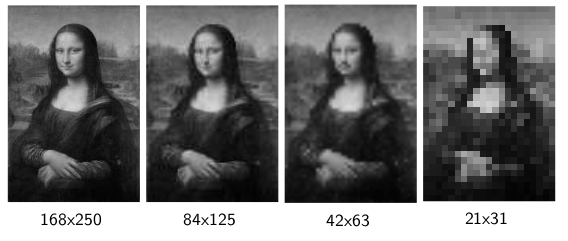
\includegraphics[width=0.7\textwidth]{img/mona_lisa_echantillon.png}
  \caption{Echantillonage spatial}
\end{figure}
\newpage
\begin{figure}[H]
  \centering
  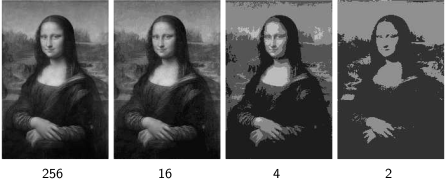
\includegraphics[width=0.7\textwidth]{img/mona_lisa_quantif.png}
  \caption{Quantification}
\end{figure}
\subsection{Notation et structure}

Pour accéder aux pixel d'une image:

\begin{itemize}
\item $w$ : nombre de colonne $i\in[0,w-1]$
\item $h$ : nombre de lignes $j\in [0,h-1]$
\end{itemize}
Ainsi $I(i,j)$ représente la valeur du pixel à la $i$ème colonne et $j$ème ligne.

Chaque pixel possède une valeur , quantifié qui peux correspondre à :
\begin{description}
\item[gris] intensité comme scalaire en $[0,2^n-1]$ où $n$ est la dynamique de l'image (la plupart du temps $n=8$)

\item[couleur] Triplet $R,G,B$ , chaque canal correspond à un 'niveau de couleur' codé de meme manière que le gris.
\end{description}

\subsection{Amélioration d'image}

\paragraph{Objectifs} Réhausser le contraste d'une image pour faire apparaitre les objets distinctements.

Pour cela on utilise des histogrammes

\subsubsection{Histogrammes d'une image}

Après quantification on peux compter les pixels de meme valeurs
\begin{defin}
  \begin{itemize}
  \item Un \emph{histogramme} est une application :
  \[
    H:
    \begin{cases}
      [0,N-1] \to [0,wh]\\
      H(z) \mapsto card(\{(x,y)\in[0,w]\times [0,h] | I(x,y) = z \})
    \end{cases}
  \]
\item On a ensuite \emph{l'histogramme normalisé} :
\[
    H_n:
    \begin{cases}
      [0,N-1] \to [01]\\
      H_n(z) \mapsto H(z)/(wh)
    \end{cases}
  \]
  L'histogramme normalisé est une distribution de proba empirique.
\item Et \emph{l'histogramme cumulé normalisé}
  \[
 H_{cn}:
    \begin{cases}
      [0,N-1] \to [0,1]\\
      H_{cn}(z) \mapsto\sum_{k=0}^{z} H_n(k)
    \end{cases}
  \]
  L'histogramme cumulé normalisé est une fonction croissante et une focntion de répartition empirique.
\end{itemize}
\end{defin}


\begin{listing}[H]
\begin{minted}{C}
  int H[N]; // histogramme
float Hn[N]; // histogramme cumulé
float Hcn[N]; // histogramme cumulé normalisé
for (i = 0; i<N; i++){
  H[i] = 0;
  Hn[i] = 0;
  Hc[i] = 0;
}
// calcul de H
for (i = 0; i<w; i++)
  for (j = 0; j<h; j++){
  int val = I(i,j);
  H[val] = H[val] + 1;
}
// calcul de Hn,Hcn
Hc[0] = Hn[0] = H[0] / (w*h);
for (i = 1; i<N; i++){
  Hn[i] = H[i] / (w*h);
  Hcn[i] = Hcn[i-1] + Hn[i];
}
\end{minted}
\caption{Calcul des histogrammes}
\end{listing}

\subsubsection{Transformation de l'histogramme}

On souhaite conserver la relation d'ordre de l'histogramme pour $I(x_1,y_1) <= I(x_2,y_2) \implies I'(x_1,y_1) <= I'(x_2,y_2)$.
Pour cela :

\begin{itemize}
\item Étalement de la dynamique via une transformation affine:
\[
  \boxed{
    z' = z'_{min} + (z'_{max}-z'_{min}) \frac{z-z_{min}}{z_{max}-z_{min}}
  }
\]
\item Quantification $z' = round(z)$

\end{itemize}

\begin{rem}
  Généralement on fais entre 0 et 255  (8 bits).
\end{rem}

Une autre possibilité et de faire de l'égalisation d'histogramme pour se rapprocher d'un histogramme cumulé uniformément croissant, cela peux passer par une transformation non linéaire.


\[
  z' = \frac{N-1}{wh}\sum_{i=0}^{z}H(i) = (N-1)H_{cn}(z)
\]


\subsection{Bruit}

\paragraph{Apparition}
\begin{itemize}
\item erreurs générant dans les pixels des valeurs différentes des valeurs réelles
\item additif, multiplicatif, impulsionnel
\item sources : capteur, transmission, interférences
\end{itemize}

\paragraph{Bruit gaussien}
\begin{itemize}
\item bon modèle pour bruit capteurs :
\[ \rho(\eta)= \frac{1}{\sqrt{2\pi}\sigma}\exp(-\frac{(\eta-\mu)^2}{2\sigma^2})\]
\item exemple en astronomie : sur l'exemple on a $\sigma=64$ (très élevé, pour des valeurs comprises entre 0 et 255). On moyenne donc sur plusieurs acquisitions pour augmenter la qualité (bruit gaussien de moyenne nulle). Pour 128 mesures, on divise l'écart-type par $\sqrt{128}$.
\end{itemize}

\paragraph{Bruit multiplicatif}
\begin{itemize}
\item images radar, laser
\item effets photochimiques (bruit "grain")
\item $I(i,j)=I_0(i,j)\eta(i,j)$ avec $E[\eta]=1$
\end{itemize}

\paragraph{Bruit convolutif}
\begin{itemize}
\item effet de flou
\item défaut de mise au point
\item mouvement rapide de la caméra
\item $I(i,j)=I_0(i,j)*g+\eta(i,j)$
\item déconvolution (Fergus et al.) : il faut avoir le mouvement ("masque") pour pouvoir déconvoluer. Par minimisation de l'énergie, on essaye de trouver cette trajectoire de l'échec.
\end{itemize}

\section{Filtrage Linéaire}
\paragraph{Caractéristiques}
\begin{itemize}
\item processus qui élimine une composante indésirable d’un signal
\item parfois utilisé pour créer un effet artistique etc.
\item en général associé à une perte d’information
\item utilise le voisinage du pixel pour calculer sa nouvelle valeur
classifications très variées :
\begin{itemize}
\item filtrage linéaire et non-linéaire
\item filtrage passe-bas, passe-bande et passe-haut
\item etc.
\end{itemize}
\end{itemize}
\subsection{Généralités}
\subsubsection{Formulation de Base (1D)}
\begin{defin}
  Un filtre linéaire réalise une opération de convolution en le signal $x(t)$ et la réponse impulsionnelle $h(t)$

  \[
    (x \star h) (t) = \int_{-\infty}^{+\infty}x(\tau)h(t-\tau)d\tau
  \]
\end{defin}
\begin{prop}
  Le produit de convolution est:
  \begin{itemize}
  \item commutatif
  \item distributif
  \item associatif
  \item Équivalent à un produit classique dans le domaine fréquentiel:
    \[
      x \star h  = \mathcal{F}^{-1}[\mathcal{F}(x)\mathcal{F}(h)]
    \]
  \end{itemize}
\end{prop}

\subsubsection{Utilisation en TI (2D discret)}

\begin{defin}
  Pour une image $I$ et un filtre $g$:

  \[
    (I\star g)(i,j) =\sum_{n=-\infty}^{+\infty}\sum_{m=-\infty}^{+\infty}I(i-n,j-m)g(n,m)
  \]
  En général le support de $g$ est compact, de dimension impaire.
\end{defin}

\subsection{Filtres courants pour réduire le bruit}

\begin{prop}[Filtre moyenneur]
  Le niveau de gris du pixel central est remplacé apr la moyenne des niveaux de gris des pixels environnants.
  \[
    w = \frac{1}{9}
    \begin{pmatrix}
      1 &1 &1\\
      1 &1 &1\\
      1 &1 &1
    \end{pmatrix}
  \]
\end{prop}
\begin{prop}[Filtre Gaussien]
le niveau de gris du pixel central est remplacé par la moyenne des niveaux de
gris des pixels environnants, pondérée par une Gaussienne 2D centrée dans ce pixel.
  \begin{itemize}
  \item filtre lisseur (donc passe-bas)
  \item  taille du support en fonction du paramètre $\sigma : l = Int + (3\sigma)$
  \item  élimine moins brutalement les hautes fréquences et préserve mieux les détails
  \end{itemize}

\end{prop}
\begin{exemple}[pour $\sigma = 0.625, l = 2$]
 \[
w = 0.4\times10^{-2}\times
\begin{pmatrix}
0.03& 0.16& 5.98& 0.16&0.03\\
0.16& 7.7 &27.8 &7.7&0.16\\
5.98& 27.8& 100 &27.8&5.98\\
0.16& 7.7 &27.8 &7.7&0.16\\
0.03& 0.16& 5.98 &0.16&0.03\\
\end{pmatrix}
\]
\end{exemple}

\begin{prop}[Filtre médian]
  \begin{itemize}
  \item remplace par la valeur médiane de tous les pixels de la fenêtre d’analyse centrée sur le pixe
  \item filtre non-linéaire, plus coûteux
  \item très bien adapté au bruit impulsionnel
\end{itemize}
\end{prop}

\subsection{Filtre de sobel}

\begin{defin}
  On défini les dérivées discrètes:
  \[
    \begin{cases}
      I_x[x,y] = I[x+1,y]-I[x-1,y]\\
      I_y[x,y] = I[x,y+1]-I[x,y-1]\\
    \end{cases}
  \]
\end{defin}
\begin{rem}
  \begin{itemize}
  \item Le calcul de la dérivé est equivalent a une convolution avec
    $\vect{-1 & 0 &1}$ resp. $\vect{-1 & 0 &1}^T$
  \item Le filtre est sensible est bruit et lisse dans la direction orthogonale.
\end{itemize}
\end{rem}


\begin{prop}[Sobel]
  On Utilise les deux filtres suivants pour déterminer les dérivées dans chacune des deux directions:
\[
  H_x =
  \begin{pmatrix}
    -1 & 0 &1 \\
    -2 & 0 &1\\
    -1 & 0 &1
  \end{pmatrix}
  \quad \quad
  H_y =
  \begin{pmatrix}
    -1 & -2&-1 \\
     0 & 0 & 0\\
     1 & 2 & 1
  \end{pmatrix}
\]


On en déduit alors la \emph{magnitude du gradient}:

\[
  \|\nabla I \| = \sqrt{(I\star H_x)^2+(I\star H_y)^2}
\]
et son \emph{orientation}:

\[
  \theta = \arctan( \frac{I \star H_y}{I \star H_x})
\]
\end{prop}
\begin{figure}[H]
  \centering
  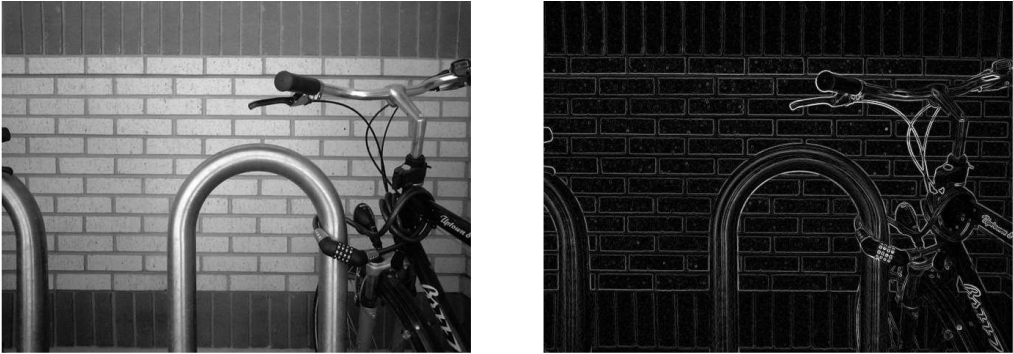
\includegraphics[width=0.7\textwidth]{img/sobel_magnitude.png}
  \caption{Echantillonage spatial}
\end{figure}

\subsection{Implémentation du filtrage}
\begin{itemize}
\item complexité d'un algorithme : très importante en systèmes embarqués
\item classes d'algorithmes :
\begin{description}
\item[sub-linéaires] en général $O(log(n))$ : optimal (par exemple dichotomie)
\item[linéaires] en $O(n)$. À noter que $O(nlog(n))$ est aussi considéré comme "rapide"
\item[autres] plus longs
\end{description}
\item séparabilité : permet de réduire le nombre d'opérations nécessaires.
\item image intégrale : calcul linéaire en nombre de pixels (en calculant à l'aide des termes précédents)
\[ \sum_{n=a}^b \sum_{m=c}^d I(n,m) = IN(b,d) - IN(a,d) - IN(b,c) + IN(a,c) \]
La somme d'un rectangle : c'est donc seulement 4 opérations si on a fait le calcul de l'image intégrale auparavant.
\end{itemize}

Petit exo : quelle est la condition pour qu'un filtre 2D soit séparable ?

\section{Filtrage pour la détection de contours}
\subsection{Filtre passe-haut : Laplacien}

\paragraph{Généralité}
\begin{defin}
  On appelle laplacien l'opérateur différentiel :
  \[
    \Delta f = \divv( \grad(f))  = \nabla\cdot \nabla f = \nabla^2 f  =  \sum_{i=1}^{n}\derivpp[f]{x_i}
  \]
  Le laplacien est  étroitement lié aux phénomènes de diffusion, il représente le taux de variation moyen de $f(x)$ sur une sphère centrée en $x$ quand la sphère varie.
\end{defin}

\begin{prop}[Laplacien d'une image]
\[ \nabla^2 I = \derivpp[I]{x_i} + \derivpp[I]{y_i} = I_{xx} + I_{yy} \]
Le masque qui correspond au calcul de $I_{xx}$ est
\[ L_{xx} = \vect{ 1 & -2 & 1} \]
On a donc le masque suivant
\[ L =
  \begin{pmatrix}
  0 & 1 & 0\\
  1 & -4 & 1\\
  0 & 1 & 0
\end{pmatrix}
\]
\end{prop}
\emph{Calcul du masque}

Développement de Taylor :
\[f(x+1) = f(x) + f'(x) + \frac{1}{2}f''(x)\]

Or, on a $f'(x)=f(x)-f(x-1)$ donc
\[ f''(x) = 2(f(x+1)-2f(x)+f(x-1) \]

\begin{rem}
  \begin{itemize}
  \item Ce masque est à symétrie centrale, ne dépend pas (en théorie) de la direction de référence.  Ce filtre est invariant par rotation.
  \item Détection de contour : passage par zéro du Laplacien. Plus le contour est net, plus l'amplitude autour de zéro du laplacien est grande.
  \item Mais le Laplacien est \emph{très} sensible au bruit.
\end{itemize}
\begin{prop}
  Pour limiter les effet du bruits on peux filtrer avec une gaussienne avant d'appliquer le laplacien.

  Avec les propriétés de la convolution on peux directement convolué avec la dérivé seconde du laplacien (LoG) fonction ``chapeau mexicain''
\end{prop}


\end{rem}

\subsection{Diffusion dans une image}

\subsubsection{Diffusion isotrope}
Le filtre Gaussien est équivalente au processus de diffusion \textbf{isotrope linéaire} suivant :
\[ \derivp[u]{t}=\divv (d\nabla u) \]

Le processus de diffusion \textbf{non linéaire isotrope} s'écrit :
\[ \derivp[u]{t}=\divv (D(x,y)\nabla u) \]

Cependant, le flux de diffusion est toujours parallèle au gradient !


Choix du coefficient de diffusion :
\[D(x,y)=\frac{1}{1+\frac{|\nabla u(x,y)|^2}{\lambda^2}}\]

$\lambda$ est le paramètre de contraste.\\

Autre coefficient possible :
\[D(x,y)=e^{\frac{|\nabla u(x,y)|^2}{\lambda^2}}\]

\subsubsection{Diffusion anisotrope} On veut diffuser perpendiculairement au gradient (selon les contours) :
\[ \derivp[u]{t}=\divv (T(x,y)\nabla u) \]

$T(x,y)$ tenseur de diffusion, dont les vecteurs propres perpendiculaires donnent les directions de diffusions, et les valeurs propres la diffusivité dans les directions respectives.

\subsubsection{Filtrage (gaussien) bilatéral}
\begin{defin}
Le filtre gaussien peux s'écrire
\[I_G(p)=\sum_{q\in S}I(q).G_{\sigma_s}(|p-q|)\]
\end{defin}

Sur un contour, la distance spatiale entre $p$ et $q$ est faible, mais la différence de poids est grande. On risque donc de faire tout baver en ne pénalisant que la distance dans l'espace image.
\begin{prop}
On fait intervenir un second terme qui pénalise la distance dans l'espace des "poids" des pixels. On empêche les pixels de valeur très différente d'intervenir dans le filtrage.
\[I_G(p)=\sum_{q\in S}I(q).G_{\sigma_s}(|p-q|).G_{\sigma_r}(|I(p)-I(q)|)\]

\end{prop}
\subsection{Application : Détection de droites}

Une fois qu'on a détecté les contours (on a une image binaire), on veut essayer de détecter des droites.\\
\begin{defin}

On représente une droite donnée par un couple de valeur $(r,\theta)$.

L'espace de représentation des droites est donc $[0,2\pi]\times[0,r_{max}]$

Équation des droites passant par $(x_0,y_0)$ : $r=x_0\cos\theta + y_0\sin\theta$
\end{defin}


On se fixe $(x_0,y_0)$ et dans l'espace de représentation des droites, l'ensemble des droites passant par $(x_0,y_0)$ est $r=x_0\cos\theta + y_0\sin\theta$ et donne une sinusoïde.

Avec un second couple $(x_1,y_1)$, on a une autre sinusoïde.\\

Pour tous les points potentiellement sur des droites, on trace les sinusoïdes dans l'espace de représentation des droites, puis on regarde les méga-intersections.

A retenir : on peut utiliser cette méthode dès qu'on peut décrire les formes par des ensembles de paramètres. On fait un système de "vote" et c'est la droite qui a le plus de votes qui est élue Miss Droite.


\subsection{Application: Detection de cercle}

De la meme manière qu'on peux détecter les droites (2 paramètres) on peux détecter des cercles avec la transformée de Hough.

\begin{defin}
  Dans cette méthode, un cercle est décrit par son équation cartésienne:
\[
    (x- a)2 + (y- b)2 = r2
\]
où le point de coordonnées $(a, b)$ est le centre du cercle et $r$ en est le rayon.
\end{defin}

\paragraph{Méthode}

Dans l'espace (a, b, r), un cercle est caractérisé par un point. L'ensemble des cercles passant par un point $M(x, y)$ donné forme un cône de sommet $(a = x, b = y, r = 0)$ et d'axe $r$. Un « bon candidat » correspond à l'intersection de plusieurs cônes.


Si le rayon est inconnu, la méthode de recherche consiste à construire une hypermatrice d'accumulation dont chaque cellule $A_{i, j, k}$ correspond à un cube de l'espace $(a, b, r)$, en balayant tous les rayons possible de 1 pixel jusqu'à la dimension de l'image.

\begin{listing}
  \inputminted{python}{hough.py}
  \caption{Création de l'accumulateur de Hough et détection des maximums}
\end{listing}

\section{Points d'intérêt}

\subsection{Nécessité de l'invariance en TI}

Les contours : traitement peu coûteux, détection robuste de courbes paramétriques mais pas suffisamment invariant.

\paragraph{Objectif} identifier des structures invariantes par rapport aux rotations, changements échelle, etc.

\subsection{Détection de coins}
\subsubsection{Les bases : Détecteur de Harris}
\begin{defin}
Un \emph{coin} est endroit de l'image qui présente une forte variation d'intensité en deux directions différentes.
\end{defin}

\paragraph{Stratégie : } Le contenu d'un patch centré dans le coin  devrait varier dans toutes les directions.

Déplacement du patch
\begin{itemize}
\item dans une zone homogène : pas coin
\item le long d'un contour : pas coin
\item près d'un coin  : coin !
\end{itemize}

On cherche donc un changement d'intensité par shift de ($\Delta x,\Delta y$):
\begin{defin}
  On utilise la fonction d'estimation de coins :
  \[
    E(x,y,\Delta x,\Delta y) = \sum_{x}^{}\sum_{y}^{}\underbracket{w(x,y)}_{support}\left[ \underbracket{I(x,y)}_{\text{Intensité}}-\underbracket{I(x+\Delta x,y+\Delta y)}_{\text{Intensite shifée}} \right]^2
  \]
  plus E est grand et plus on a de chance de trouver un coin.
\end{defin}

Cette methode est lourde en calcul et peux etre rendu plus rapide:

\begin{prop}
  En faisant une approx au premier ordre de la fonction on a :

\[
  E(x,y) =  \vect{\Delta x & \Delta y}
  \underbrace{\begin{bmatrix}
    <I_x^2> & <I_xI_y> \\
    <I_xI_y> & <I_y^2>
  \end{bmatrix}}_{\text{ tenseur de structure}}
 \vect{\Delta x \\ \Delta y}
\]
\end{prop}

\begin{rem}
Le tenseur de structure est composé des dérivée de l'image sur le patch moyennée. Les vecteurs propres indiquent les direction principales de variation de gradient
dans le voisinage du point (voir l’ellipse du changement constant)
\end{rem}

\paragraph{Méthode} :
On peux calculer $\lambda_1$ et $\lambda_2$ explicitement mais c'est lourd. On préfère utiliser :
\[
  R = \det(M) - \alpha tr(M)^2 = \lambda_1\lambda_2 -\alpha(\lambda_1+\lambda_2)^2
\]

Et on choisi $\alpha \in[0.04; 0.06]$. Les valeurs propres intéressante sont alors des maximums locaux de $R$.

\paragraph{Algorithme}
\begin{itemize}
\item Calcul des gradients  gaussien de l'image
\item Calcul du tenseur des structures
\item Calcul de $R$
\item Seuillage et suppression des valeurs non maximales.
\end{itemize}
\begin{listing}
  \inputminted{python}{harris.py}
\end{listing}


\paragraph{Comment gérer le changement d'échelle ?} Algorithme qui détecte en chaque endroit de l'image l'échelle qui ferait que cet endroit serait un coin.


\subsection{Détecteur FAST}
\subsection{Détecteur SIFT}





\section{La couleur}

\subsection{Les descripteurs}

En niveaux de gris, le descripteur le plus simple est la luminosité. Un autre descripteur possible (Local Binary Pattern LBP) prend le voisinage 3x3 d'un pixel et fait un seuil des valeurs des pixels par rapport au pixel central.

En couleurs, c'est plus complexe car il y a 3 canaux.\\

La couleur n'est pas forcément un atout car l'information supplémentaire n'est pas nécessairement un atout. En général, les algorithmes de traitement de couleurs sont construits pour des applications particulières : par exemple, suppression fond vert.\\

\paragraph{Capteurs RGB} on peut difficilement réaliser un système permettant de séparer les canaux pour les envoyer sur 3 capteurs différents. On réalise donc une matrice du type :

\begin{center}
\begin{tabular}{cccccc}
R & V & R & V & R & V \\
V & B & V & B & V & B \\
R & V & R & V & R & V \\
V & B & V & B & V & B \\
\end{tabular}
\end{center}

En 1 point donné, on interpole entre les données voisines pour les différents canaux.
Il y a plus de capteurs verts car c'est la couleur à laquelle l'oeil humain est le plus sensible.\\

Avantage : l'image RGB a donc la taille d'une image en niveaux de gris. \\

Inconvénient : sur les contours, on aura des aberrations à cause des interpolations. Par exemple, à la frontière entre une zone rouge et une zone verte, on fera apparaître du jaune.

\paragraph{Sources lumineuses} on caractérise la lumière de manière spectrale, et on a don une grande variétés de spectres d'émission selon les sources. Donc en ne changeant ni l'objet, ni l'observateur, on peut avoir de grandes différences dans ce qui sera observé en fonction de l'éclairage "ambiant".

\paragraph{Perception} l'important n'est pas ce qui compose l'environnement mais la manière dont on le perçoit. Par exemple : un damier sur laquelle une ombre est projetée, le cerveau humain sait que les carrés blancs sont toujours plus foncés que les gris, mais ce n'est pas forcément vrai entre un carré blanc "à l'ombre" et un carré gris dans la lumière.

\paragraph{Descripteurs} principe de la trichromie : 3 couleurs primaires permettent de reproduire la quasi-totalité des couleurs

\begin{itemize}
\item Observateur standard RGB 1931 : il existe une partie négative de la partie rouge, qui n'est pas cohérente avec la théorie additive.
\item Observateur standard CIE 1931 :
  \[ \vect{ X \\ Y \\ Z } = \frac{1}{0.17697}
    \begin{bmatrix}
    0.49 & 0.31 & 0.20\\
    0.17697 & 0.81240 & 0.01063\\
    0 & 0.01 & 0.99
  \end{bmatrix}
    \vect{ R \\ G \\ B } \]
Le $Y$ est proche du $V$, le $Z$ est proche du $B$.
\end{itemize}

\subsection{Seuillage optimal méthode de Otsu}

la méthode d'Otsu est utilisée pour effectuer un seuillage automatique à partir de la forme de l'histogramme de l'image1, ou la réduction d'une image à niveaux de gris en une image binaire. L'algorithme suppose alors que l'image à binariser ne contient que deux classes de pixels  puis calcule le seuil optimal qui sépare ces deux classes afin que leur variance intra-classe soit minimale.

\begin{prop}
  On cherche le seuil $t$ tel que :
  \[
     t = \arg\max_{t} \omega_1(t)\omega_2(t)[\mu_1(t)-\mu_2(t)]^2
  \]
  Avec:
  \begin{itemize}
  \item $\omega_1(t) = \sum_{i=0}^{t}H_n(i)$ et $\omega_2(t)= \sum_{i=t+1}^{N-1}H_n(i)$
  \item $\mu_1(t) = \frac{1}{\omega_1(t)}\sum_{i=0}^{t} i \cdot H_n(i)$. et $\mu_2 =  \frac{1}{\omega_2(t)}\sum_{i=t+1}^{N-1} i \cdot H_n(i)$
  \item .
  \end{itemize}
\end{prop}
\section{Estimation}

À partir d'une image on cherche à estimer un ensemble $\theta$ de paramètres (déplacememt, état d'un d'un système )

\paragraph{Source du problème}
On ne pas ignorer les outliers et déterminer les paramètre du modèle. Les methodes de tyoe moindres carré sont très sensibles aux outliers à cause de la fonction d'erreur quadratique associée.

Différentes approches sont possibles:

\subsection{Analyse de l'ensemble des résidus}

On utilise des variation de la méthode des moindres carrés:

\begin{prop}[Least Median of Squares]
  On remplace la somme par la médiane :
  \[
    \theta = \arg\min_{\theta}~\text{med } \rho(r_i)
  \]
\end{prop}

\begin{prop}[Least Trimmed Squares]
  On tri les résidus et on en sélectionne $M$ où $N/2 < M< N$.
  \[
    \theta \arg \min \sum_{i=0}^{M}\rho(r_i)
  \]
\end{prop}

Une autre alternative est d'utilisé une autre fonction de cout (cf UE 451),qui doit rester symétrique définie positive

\subsection{RANSAC}
\begin{defin}
``  RANSAC, abréviation pour RANdom SAmple Consensus, est une méthode pour estimer les paramètres de certains modèles mathématiques. Plus précisément, c'est une méthode itérative utilisée lorsque l'ensemble de données observées peut contenir des valeurs aberrantes (outliers). Il s'agit d'un algorithme non-déterministe dans le sens où il produit un résultat correct avec une certaine probabilité seulement, celle-ci augmentant à mesure que le nombre d'itérations est grand. L'algorithme a été publié pour la première fois par Fischler et Bolles en 1981''
\end{defin}

\begin{figure}[H]
  \centering
  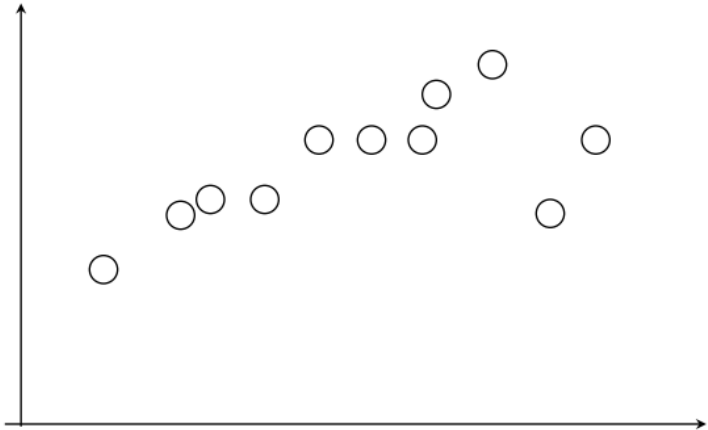
\includegraphics[width=0.3\textwidth]{img/ransac_0.png}%
  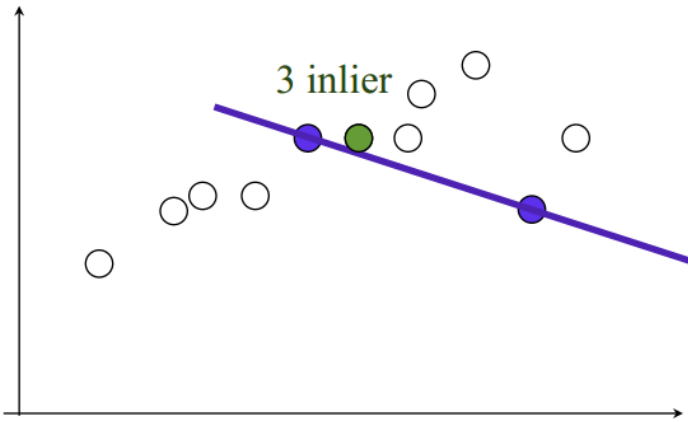
\includegraphics[width=0.3\textwidth]{img/ransac_1.png}
  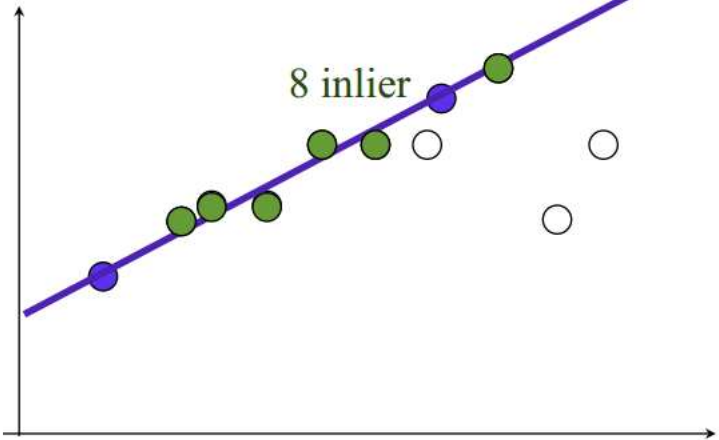
\includegraphics[width=0.3\textwidth]{img/ransac_2.png}%
  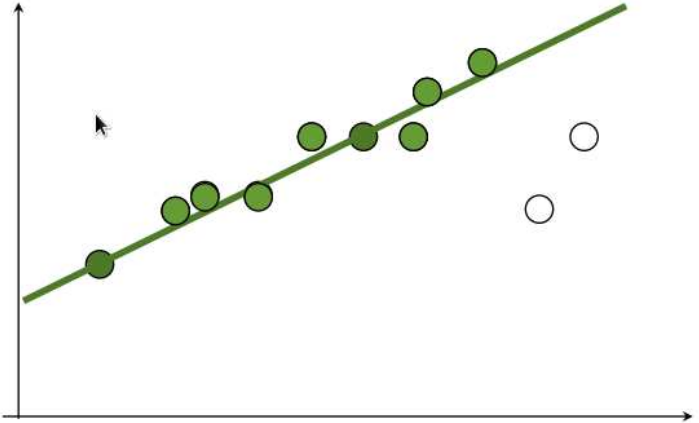
\includegraphics[width=0.3\textwidth]{img/ransac_3.png}
  \caption{Méthode RANSAC}
\end{figure}
\newpage
\paragraph{Algorithme}~\\
\textbf{entrées :}\vspace{-1em}
\begin{verbatim}
    data   - un ensemble d'observations
    modele - un modèle qui peut être ajusté à des données
    n      - nb min de données nécessaires pour ajuster le modèle
    k      - nb max d'itérations de l'algorithme
    t      - seuil d'appartenance au modèle
    d      - seuil de données nécessaire pour valider le modèle
\end{verbatim}
\textbf{sorties :}\vspace{-1em}
\begin{verbatim}
    meilleur_modèle - les paramètres du modèle qui correspondent le mieux aux données
    meilleur_ensemble_points - données à partir desquelles ce modèle a été estimé
    meilleure_erreur - l'erreur de ce modèle par rapport aux données
\end{verbatim}

\begin{listing}[H]
\begin{verbatim}
itérateur := 0
meilleur_modèle := aucun
meilleur_ensemble_points := aucun
meilleure_erreur := infini
tant que itérateur < k
    points_aléatoires := n valeurs choisies au hasard à partir des données
    modèle_possible := paramètres du modèle correspondant aux points_aléatoires
    ensemble_points := points_aléatoires

    Pour chaque point des données pas dans points_aléatoires
        si le point s'ajuste au modèle_possible avec une erreur inférieure à t
            Ajouter un point à ensemble_points

    si le nombre d'éléments dans ensemble_points est > d
        (ce qui implique que nous avons peut-être trouvé un bon modèle,
        on teste maintenant dans quelle mesure il est correct)
        modèle_possible := paramètres du modèle réajusté sur ensemble_points
        erreur := ecart entre données et modèle.
        si erreur < meilleure_erreur
            (nous avons trouvé un modèle qui est mieux que tous les précédents,
            le garder jusqu'à ce qu'un meilleur soit trouvé)
            meilleur_modèle := modèle_possible
            meilleur_ensemble_points := ensemble_points
            meilleure_erreur := erreur

    incrémentation de l’itérateur

retourne meilleur_modèle, meilleur_ensemble_points, meilleure_erreur
\end{verbatim}
\caption{Algorithme de la méthode randsac}
\end{listing}


\subsection{La segmentation}
\emph{poly de l'ENSTA très bien fait}

La segmentation consiste à regrouper les différents pixels de l'image en un nombre (donné) de région (peut aussi consister a une taille de région maximale, les deux, etc...). En pratique on réalise une partition de l'image

\subsection{Segmentation par découpage}
\begin{defin}
  L'idée des algorithmes de type « Split \& Merge » est de produire
    automatiquement une partition initiale en régions petites (Split), qui vont ensuite croître en se regroupant (Merge)
  \begin{itemize}
  \item  La partition initiale (Split) est  réalisée en \emph{divisant récursivement} l'image en régions de tailles identiques lorsqu'un certain critère d'homogéneité n'est pas satisfait: \emph{$R$ est divisée} (ex: si $\sigma_R> seuil$)

  \item  Lors de cette phase, le graphe d'adjacence, ou Region Adjacency Graph (RAG) est créé :  à chaque région est associé un sommet du graphe, et des arêtes relient les sommets correspondants à deux régions qui se touchent.
  \item La \emph{phase de regroupement} (Merge) utilise le RAG pour modifier la partition initiale : pour chaque sommet R du RAG, on cherche s'il existe un sommet $R'$ voisin dans le RAG et de valeur suffisamment proche, et si c'est le cas, on les fusionne:
 $R et R'$ sont fusionnées si $\mu_{R}-\mu_{R'} < seuil$
\end{itemize}
\end{defin}

\paragraph{Phase de découpage}

Lors de la phase de découpage on forme le quadtree et le graphe d'adjacence:

\begin{figure}[H]
  \centering
  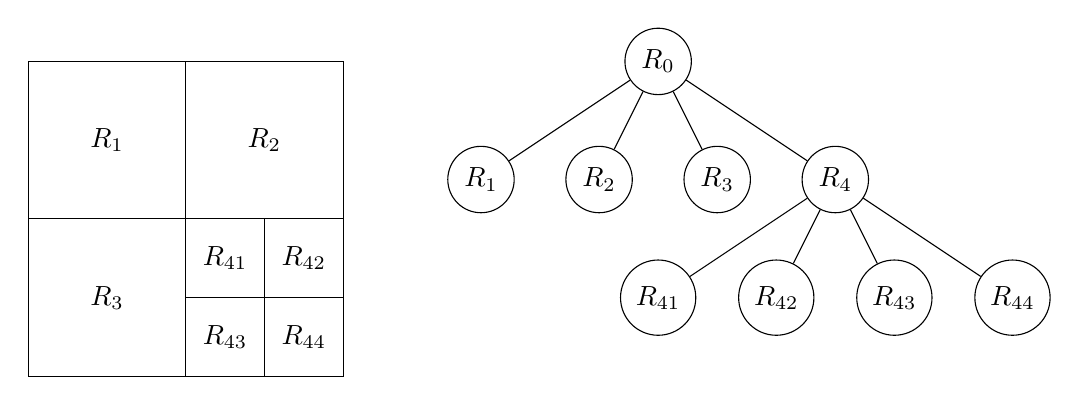
\begin{tikzpicture}
    \begin{scope}
      \draw (0,0) rectangle ++ (4,4);
      \draw (2,0) --  ++ (0,4) (0,2) -- ++(4,0);
      \draw (3,0) -- ++(0,2) (2,1) -- ++ (2,0);
      \draw (1,1) node{$R_3$}
      (1,3) node{$R_1$}
      (3,3) node{$R_2$}
      (2.5,1.5) node{$R_{41}$}
      (3.5,1.5) node{$R_{42}$}
      (2.5,0.5) node{$R_{43}$}
      (3.5,0.5) node{$R_{44}$};
    \end{scope}
    \begin{scope}[shift={(8,4)},
      every node/.style = {shape=circle, draw}]
      \node{$R_0$}
      child{ node {$R_1$}}
      child{ node {$R_2$}}
      child{ node {$R_3$}}
      child{ node {$R_4$}
        child{ node {$R_{41}$}}
        child{ node {$R_{42}$}}
        child{ node {$R_{43}$}}
        child{ node {$R_{44}$}}};
    \end{scope}
  \end{tikzpicture}
  \caption{Quadtree et graphe d'adjacence}
\end{figure}
\begin{rem}
  L'algorithme de découpage est implantable très facilement de manière récursive
\end{rem}


\subsection{Segmentation par optimisation}
\begin{prop}
Cette fois ci on cherche à déterminier la fonction $f$ bidimensionnelle, constante par morceaux (une valeur , une région) proche
de l’image I , avec une partition simple du point de vue géométrique. Pour cela on utilise la fonctionnelle de cout :
\[
  K = \sum_{i}^{} \iint_{R_i}(I(x,y)-f_i)\d x \d y + \mu \sum_{j}^{}\int_{\Gamma_j}^{}dl
\]
où $\Gamma_j$ sont les portions de contour entourant la région de la région
\end{prop}

\begin{rem}
  Il n'existe pas de solution directe au problème de minimisation. Il y a deux techniques pour approcher la solution:
  \begin{itemize}
  \item méthodes variationnelles sur des courbes fermées
  \item méthodes markoviennes par itération à partir d’une segmentation initiale
  \end{itemize}
\end{rem}
\paragraph{méthode variationnelles}
On utilise une fonction de cout $E = E_i+E_e$ tel que
\begin{itemize}
\item $  E_i = \int_{0}^{1}\alpha (C'(s))^2ds$ pénalise la longueur du contour (``snake'')
\item $E_e = \int_{0}^{1}-\nabla I(x(s),y(s))ds$ favorise l'alignement sur les forts gradients.
\end{itemize}

\paragraph{Technique markoviennes}

On teste les changements de pixel/sous-région  d'une région à une autre, et on prend le meilleur (ie qui minimise la fonctionnelle). Pour cela on part souvent d'une sur-segmentation.


\section{La classification}
\paragraph{Objectif}:
\begin{itemize}
\item Obtenir une représentation simplifiée mais pertinente des données originales
\item Mettre en évidence les similiratité entre les objets.
\end{itemize}

\paragraph{Problématique de la visualisation des données}

Il est difficile de se représenter la classification de manière ``brute'' au dela de 5 paramètres on peux utiliser l'analyse en composante principale (par réduction de la dimension) ou l'analyse linéaire discriminante.


\subsection{Analyse en composantes principales}
\begin{itemize}
\item indispensable quand le nombre de variables est très grand
\item analyse de la variabilité / dispersion des données
\item objectif : décrire à partir de q < d dimensions cette variabilité
\item réduction des données a q nouveaux descripteurs
\item visualisation si q = 2 ou q = 3
\item interprétation des données : liaisons inter-variables
\end{itemize}

\paragraph{Algorithme}

\begin{enumerate}
\item recentrage des données $\vec{X} = (\vec{x}-\mu)^T$.
\item Calcul de la matrice de covariance $\Sigma$.
\item diagonalisation de $\Sigma$ et classement par valeur propres croissantes.
\item sélection des $q$ premiers vecteurs propres $C_k$
\item Calcul des valeur réduites $a_i$ qui remplacent $x_i$ par $a_{ik}= <x_i,C_k>$
\end{enumerate}

\begin{rem}
  Le PCA ne prend pas en compte la notion de classe. on peux aussi utiliser l'analyse linéaire discriminante.
\end{rem}
\subsection{Analyse linéaire discriminante}

\paragraph{Algorithme}
\begin{enumerate}
\item recentrage des données $\vec{X}=(\vec{x}-\mu)^T$
\item Calcul de la matrice de covariance $\Sigma$.
\item Calcul de la matrice de covariance interclasse $\vec{B}$.
  \[
    \vec{B} = \sum_{k=1}^{c}n_k\frac{(\mu_k-\mu)(\mu_k-\mu\rangle)^T}{n}
  \]
  où $k$ représente la classe
\item diagonalisation de $\Sigma^{-1}\vec{B}$ et classement par valeur propres croissantes
\item sélection des $q$ premiers vecteurs propres $C_k$.
\item Calcul des valeurs réduites $\vec{a_i}$ qui remplacent $x_i$ par $a_{ik}=<x_i,C_k>$
\item classification d'une nouvelle observation par la distatnce au centroïde le plus proche.
\item classification linéaire : médiane entre les centroïdes.
\end{enumerate}


\subsection{Intégration de la connaissance}
\subsection{Classification non supervisée - K-means}

on cherche à déterminer des ``clusters''  dans les observations. En minimisant
\[
 \min_{\mu_1....\mu_k} \sum_{i=1}^{k}\sum_{x_j\in C_i}^{} (x_j-\mu_i)^2
\]

\paragraph{Fonctionnement}
\begin{verbatim}
choose mu_i , i in [1 k] // initialisation
while (any mu_i changes){
  assign all x_j to closest mu
  update mu_i , i in [1 k]
}
\end{verbatim}
À chaque itération la fonction objectif diminue. c'est rapide et parallèlisable.





\end{document}

%%% Local Variables:
%%% mode: latex
%%% TeX-master: "main"
%%% End:
